\section{Sistema C – Sistema Acesso ao Estacionamento}


Quando é pressionado o botão "seta para cima" no comando, o servo faz com que o portão abra.

\begin{figure}[H]
    \centering
    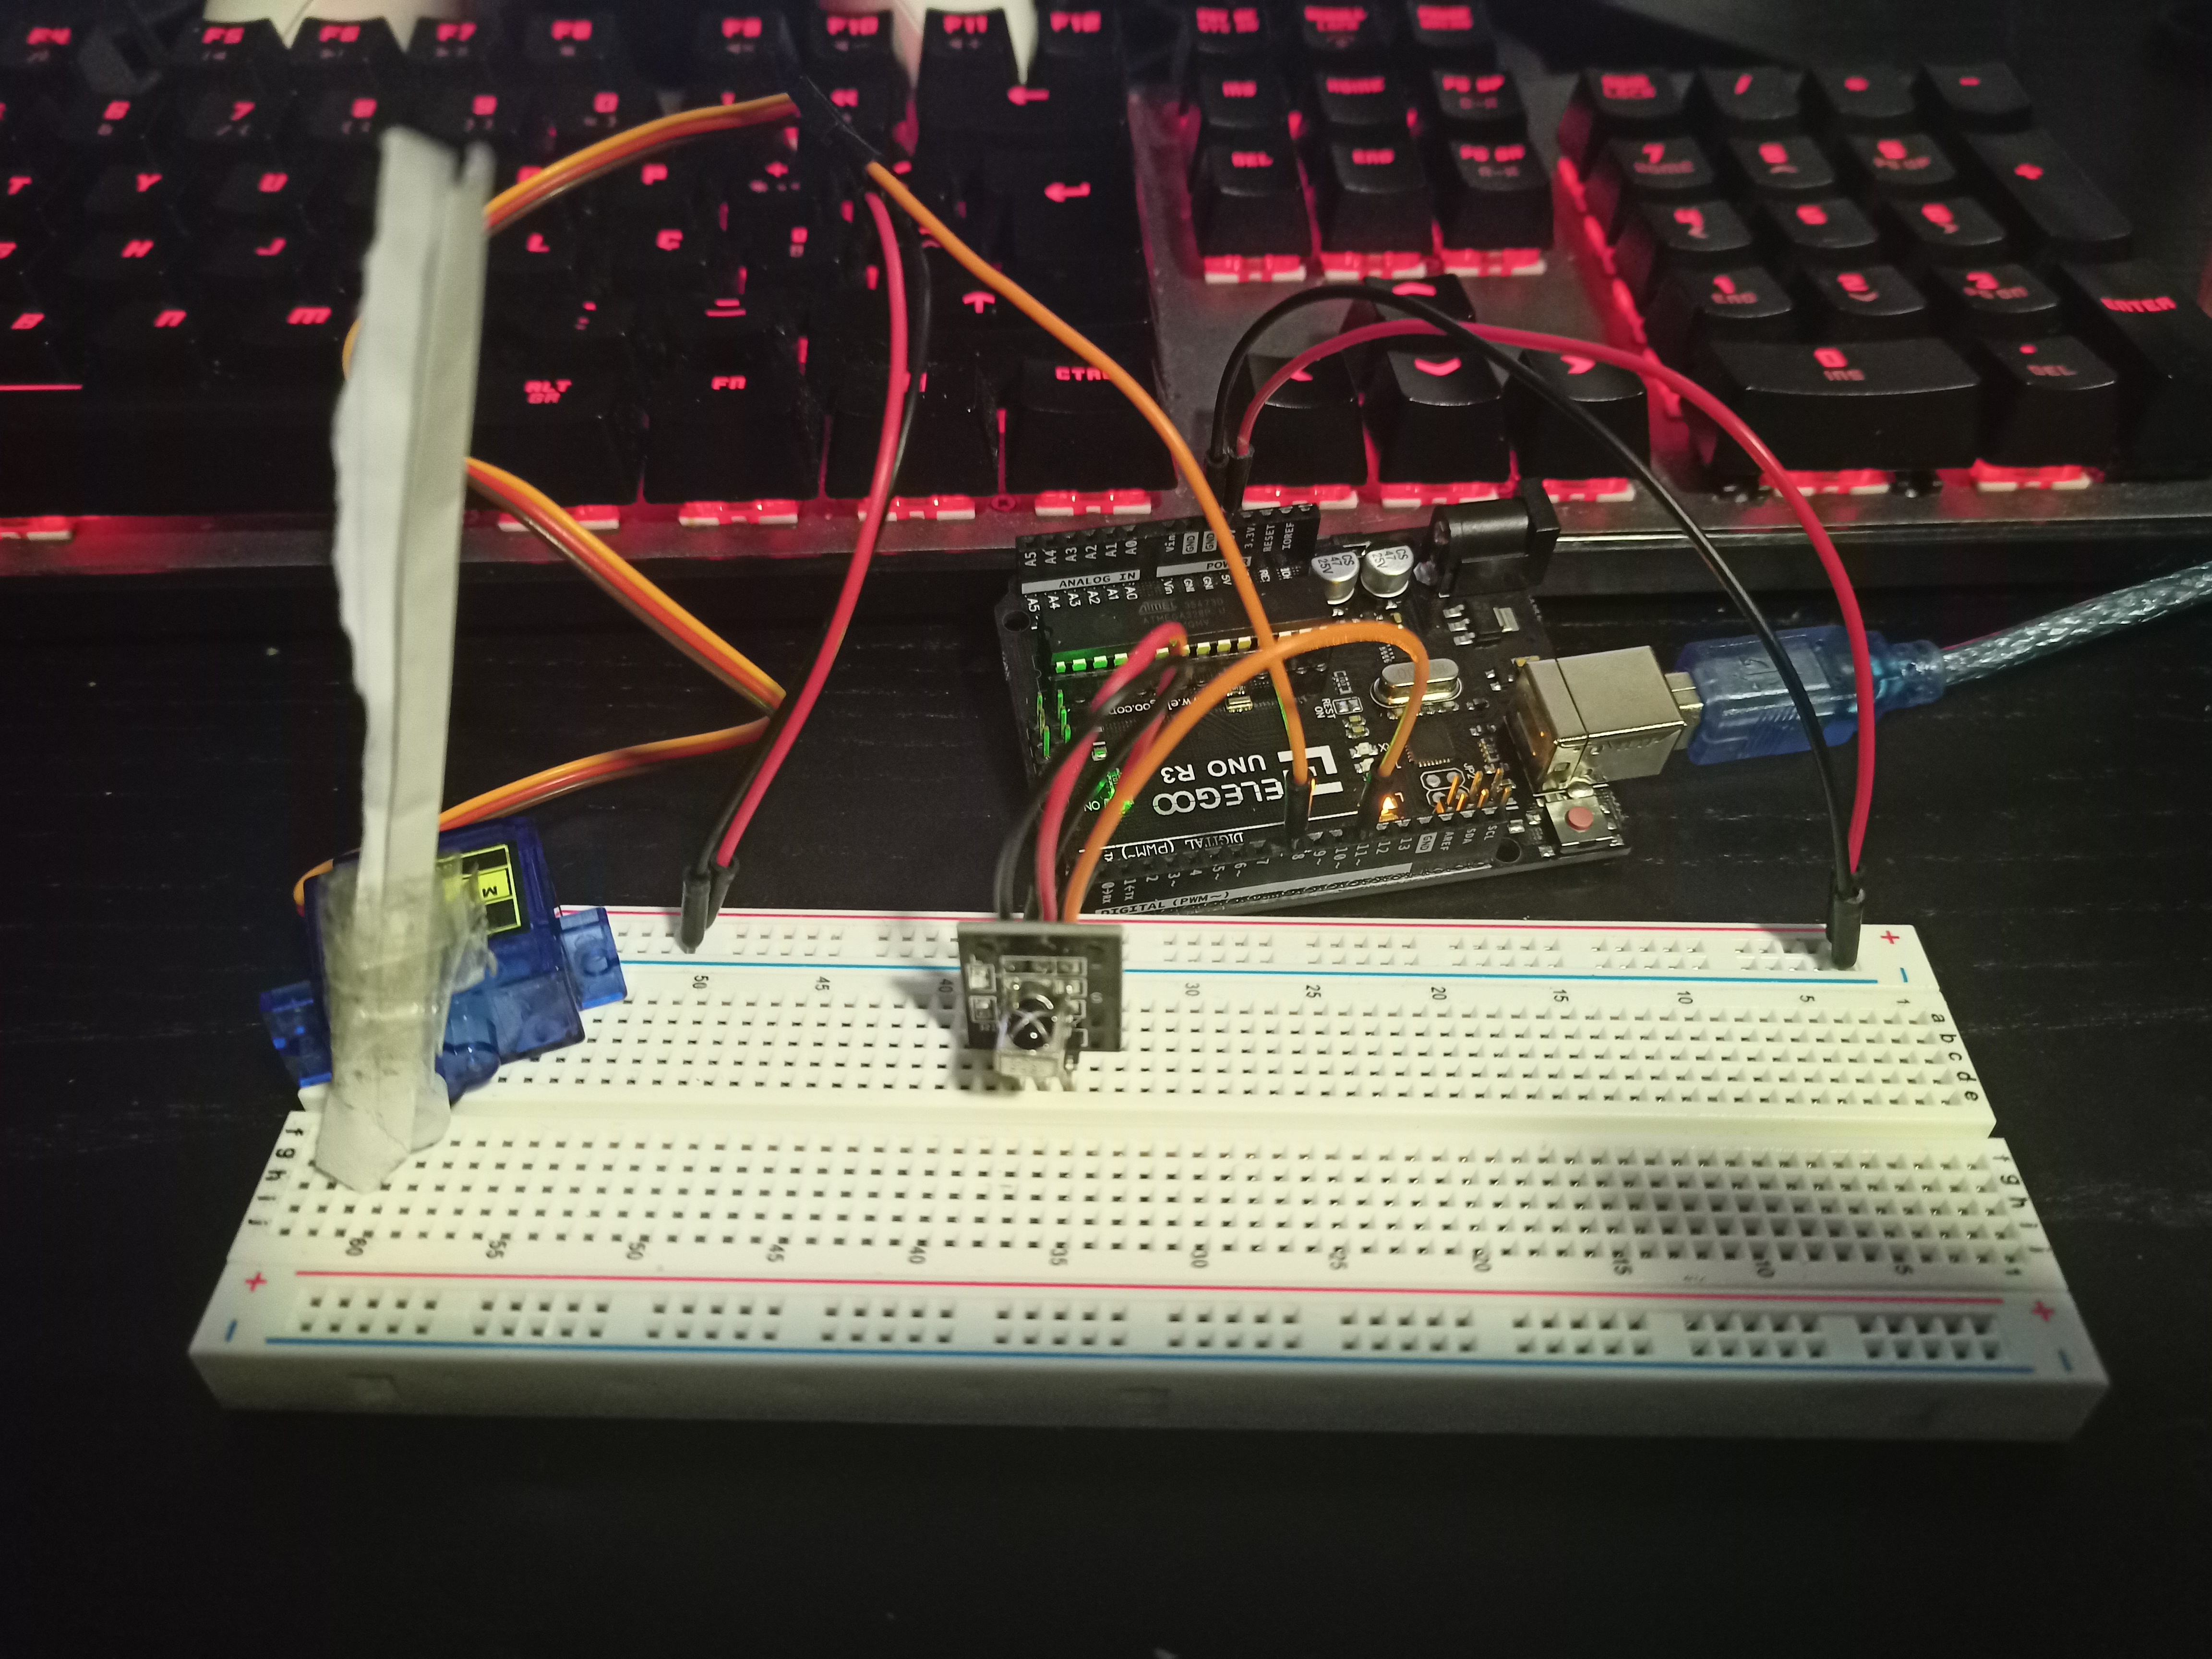
\includegraphics[scale=0.03]{images/testes/sisC_Open.jpg}
    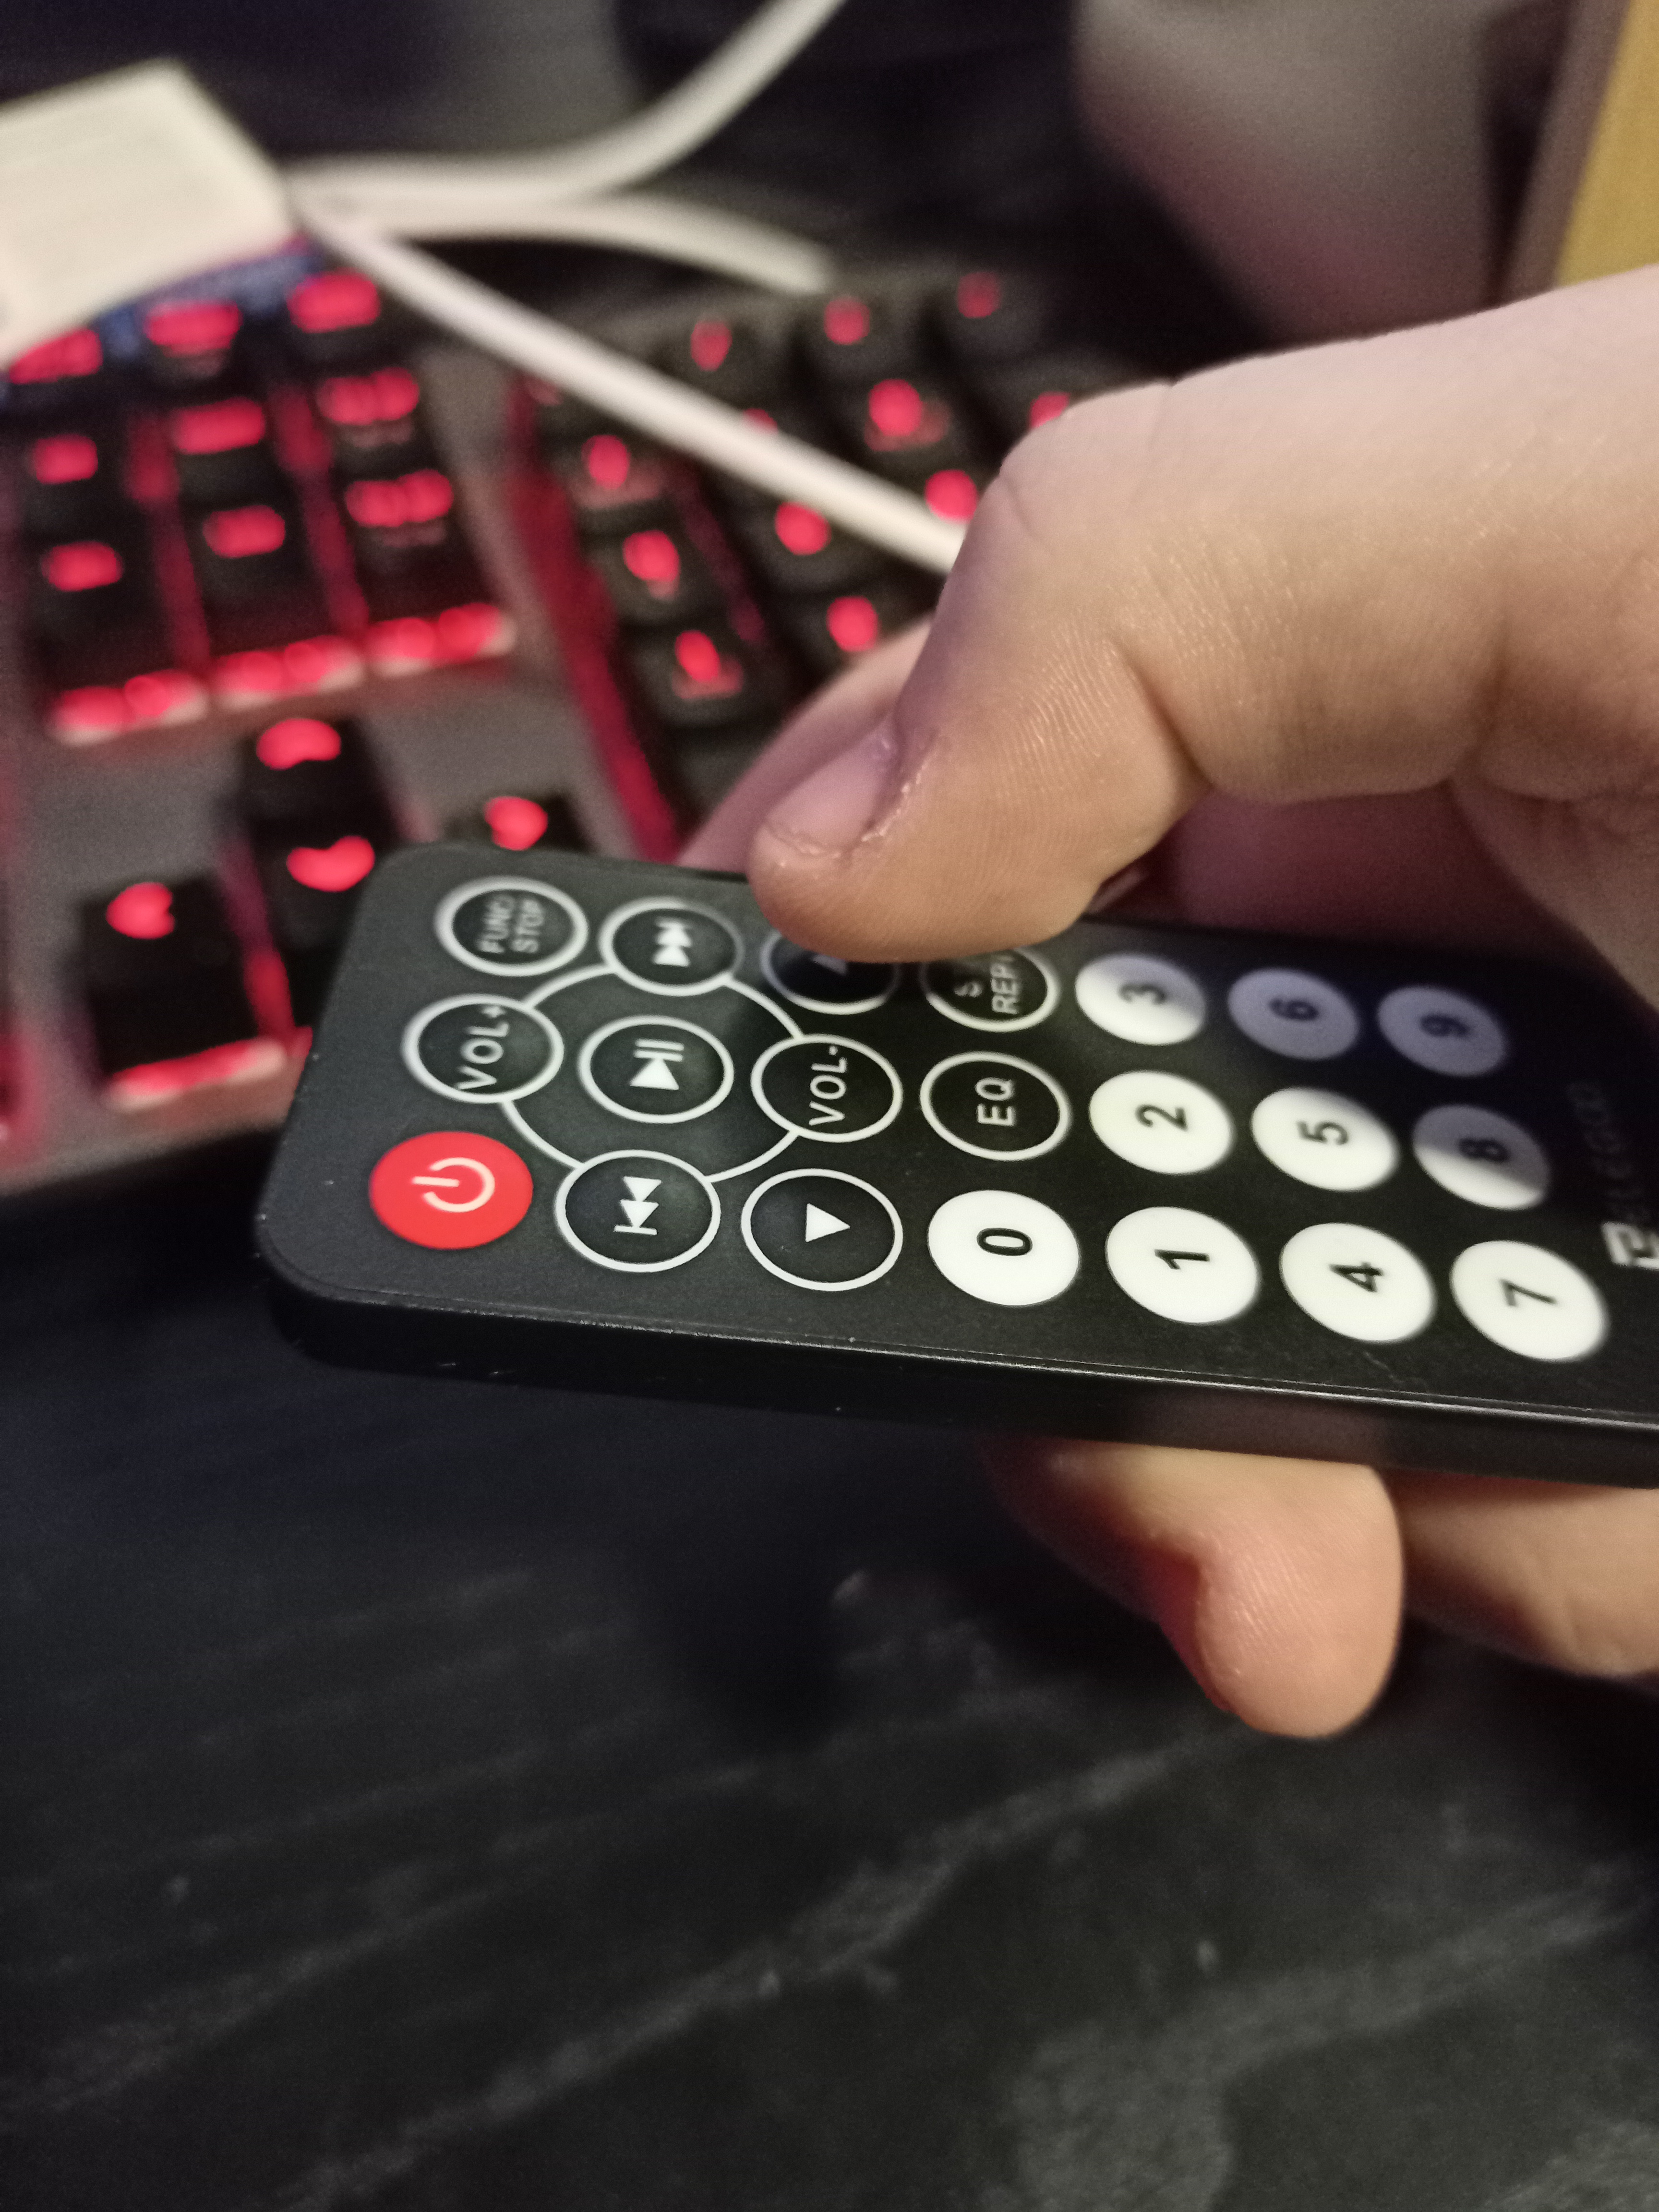
\includegraphics[scale=0.0225]{images/testes/ControllerUp.jpg}
    \selectlanguage{portuguese}\caption{Portão Aberto}
\end{figure}


Quando é pressionado o botão "vermelho" no comando, o servo suspende o seu movimento.

\begin{figure}[H]
    \centering
    
    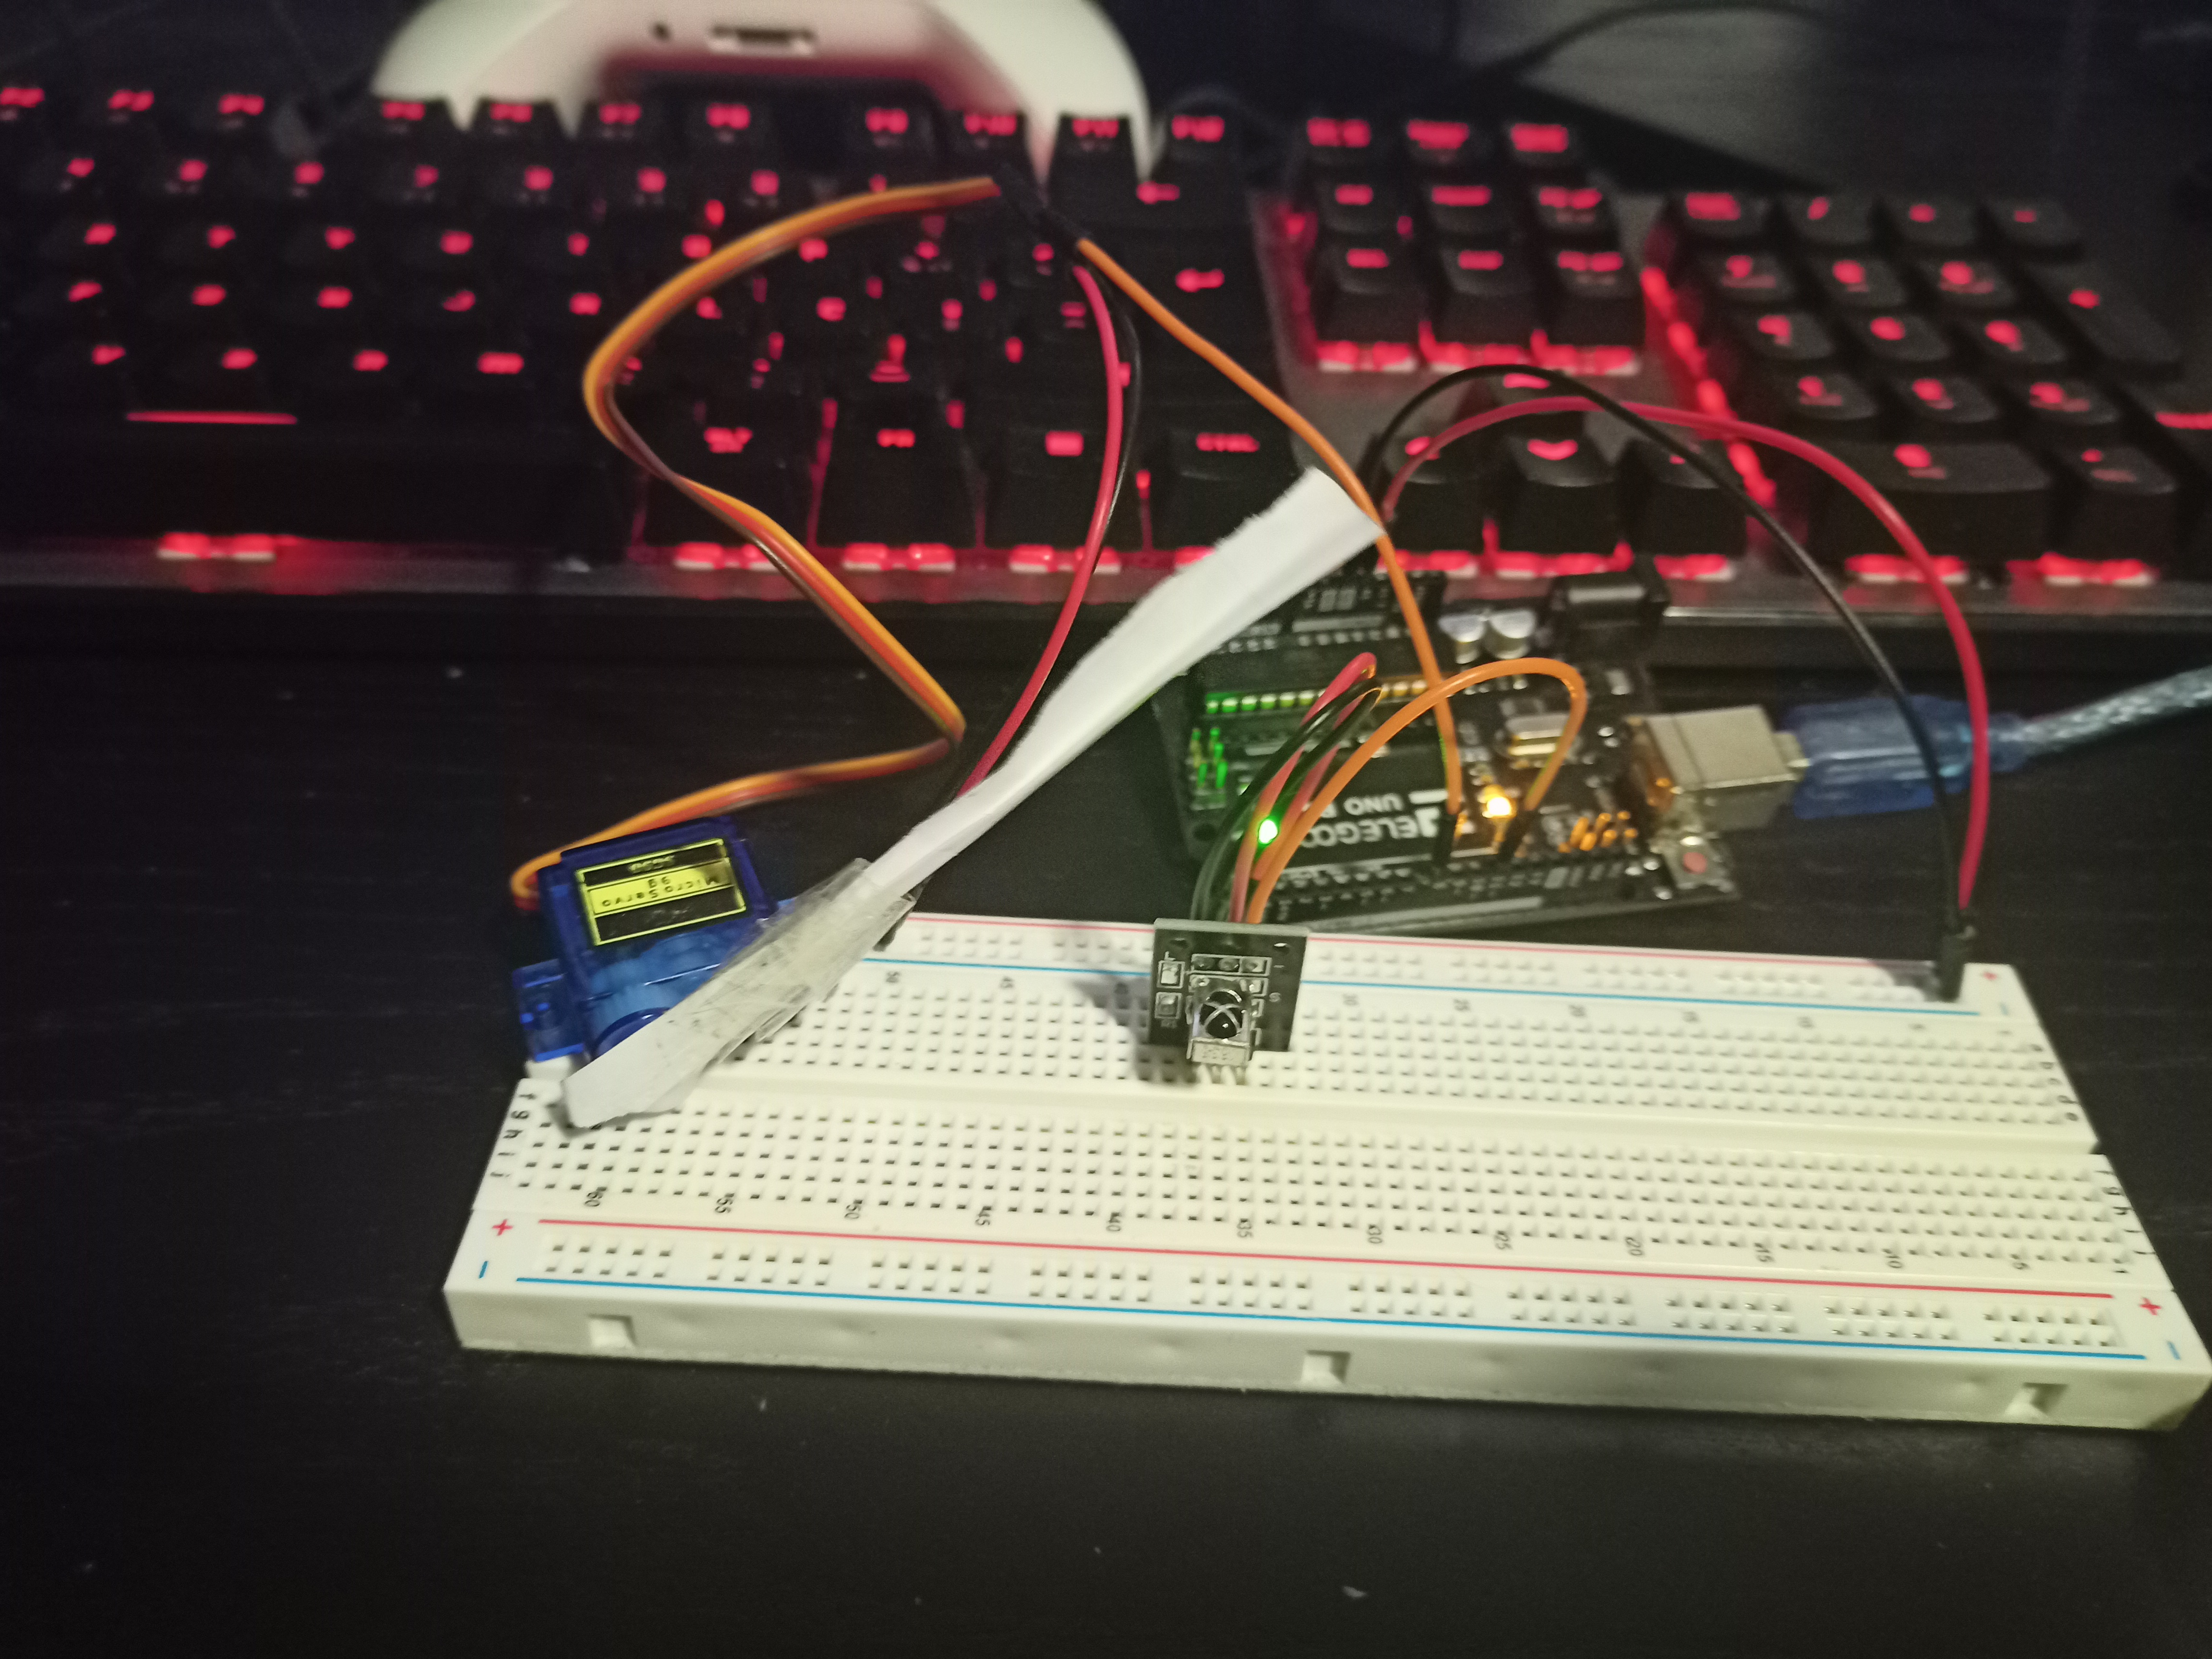
\includegraphics[scale=0.03]{images/testes/sisC_semiOpen.jpg}
    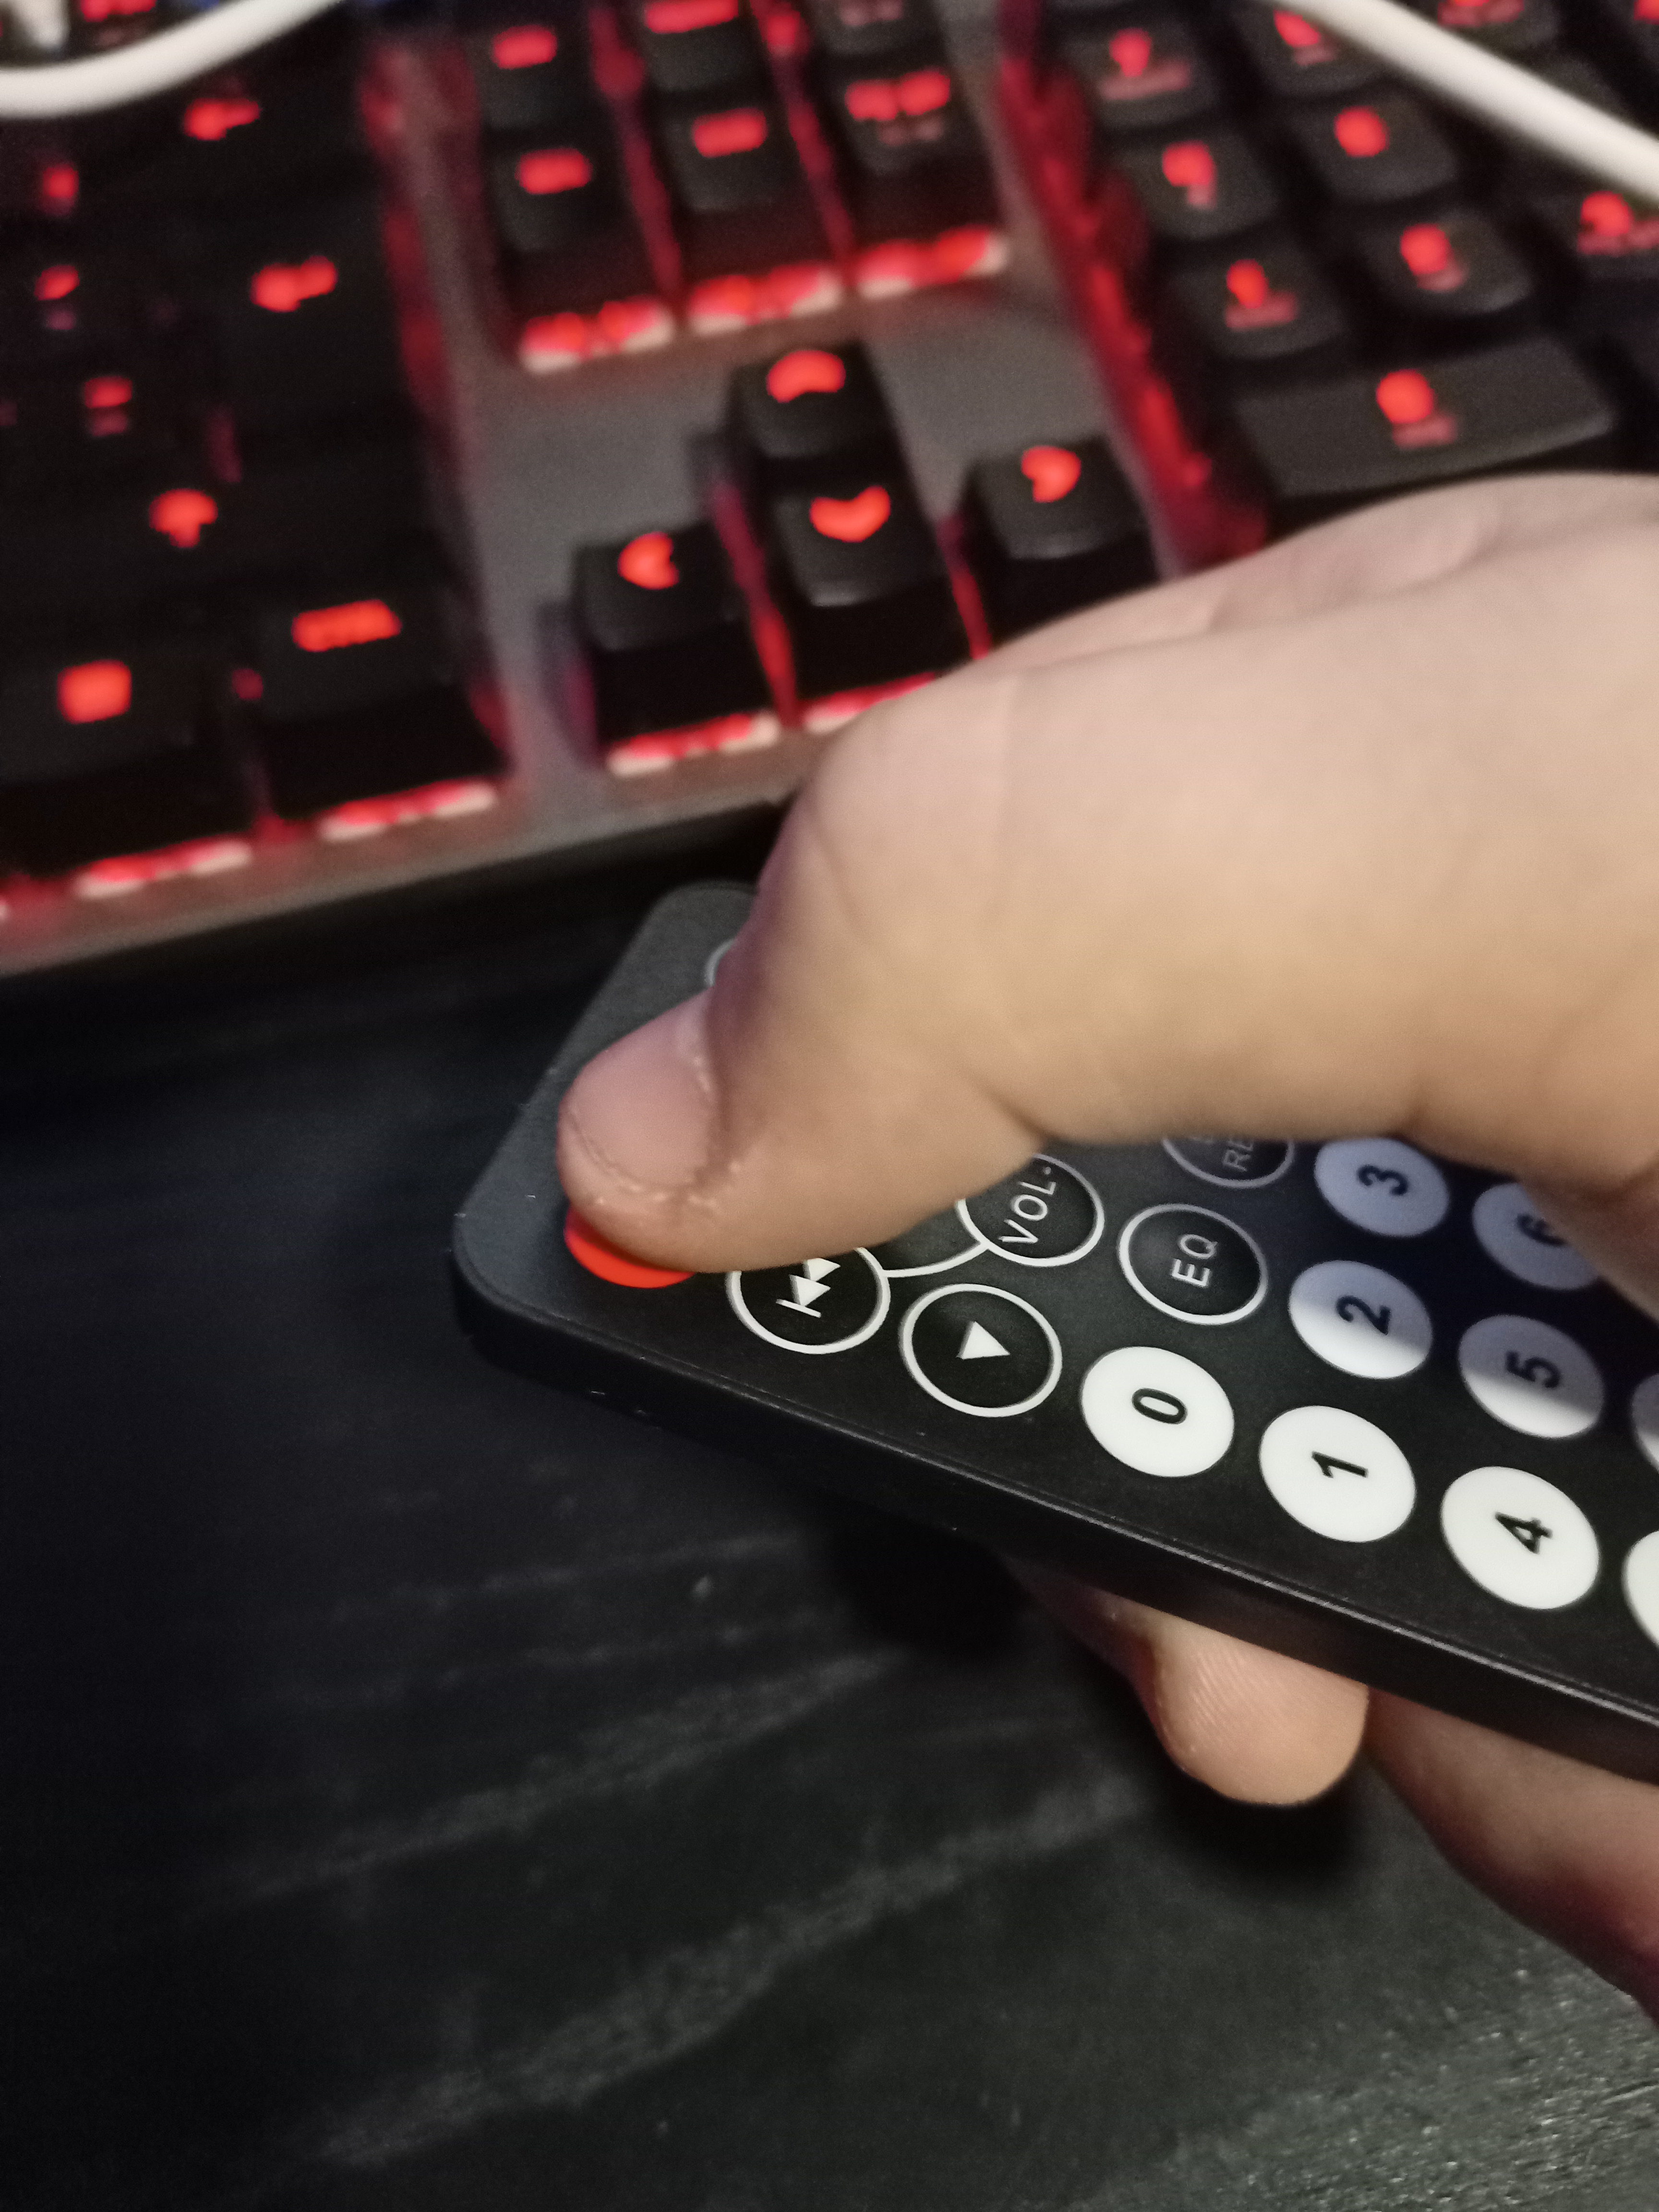
\includegraphics[scale=0.0225]{images/testes/controllerOff.jpg}
    \selectlanguage{portuguese}\caption{Portão Semi-aberto}
\end{figure}


Quando é pressionado o botão "seta para baixo" no comando, o servo faz com que o portão feche.

\begin{figure}[H]
    \centering
    
    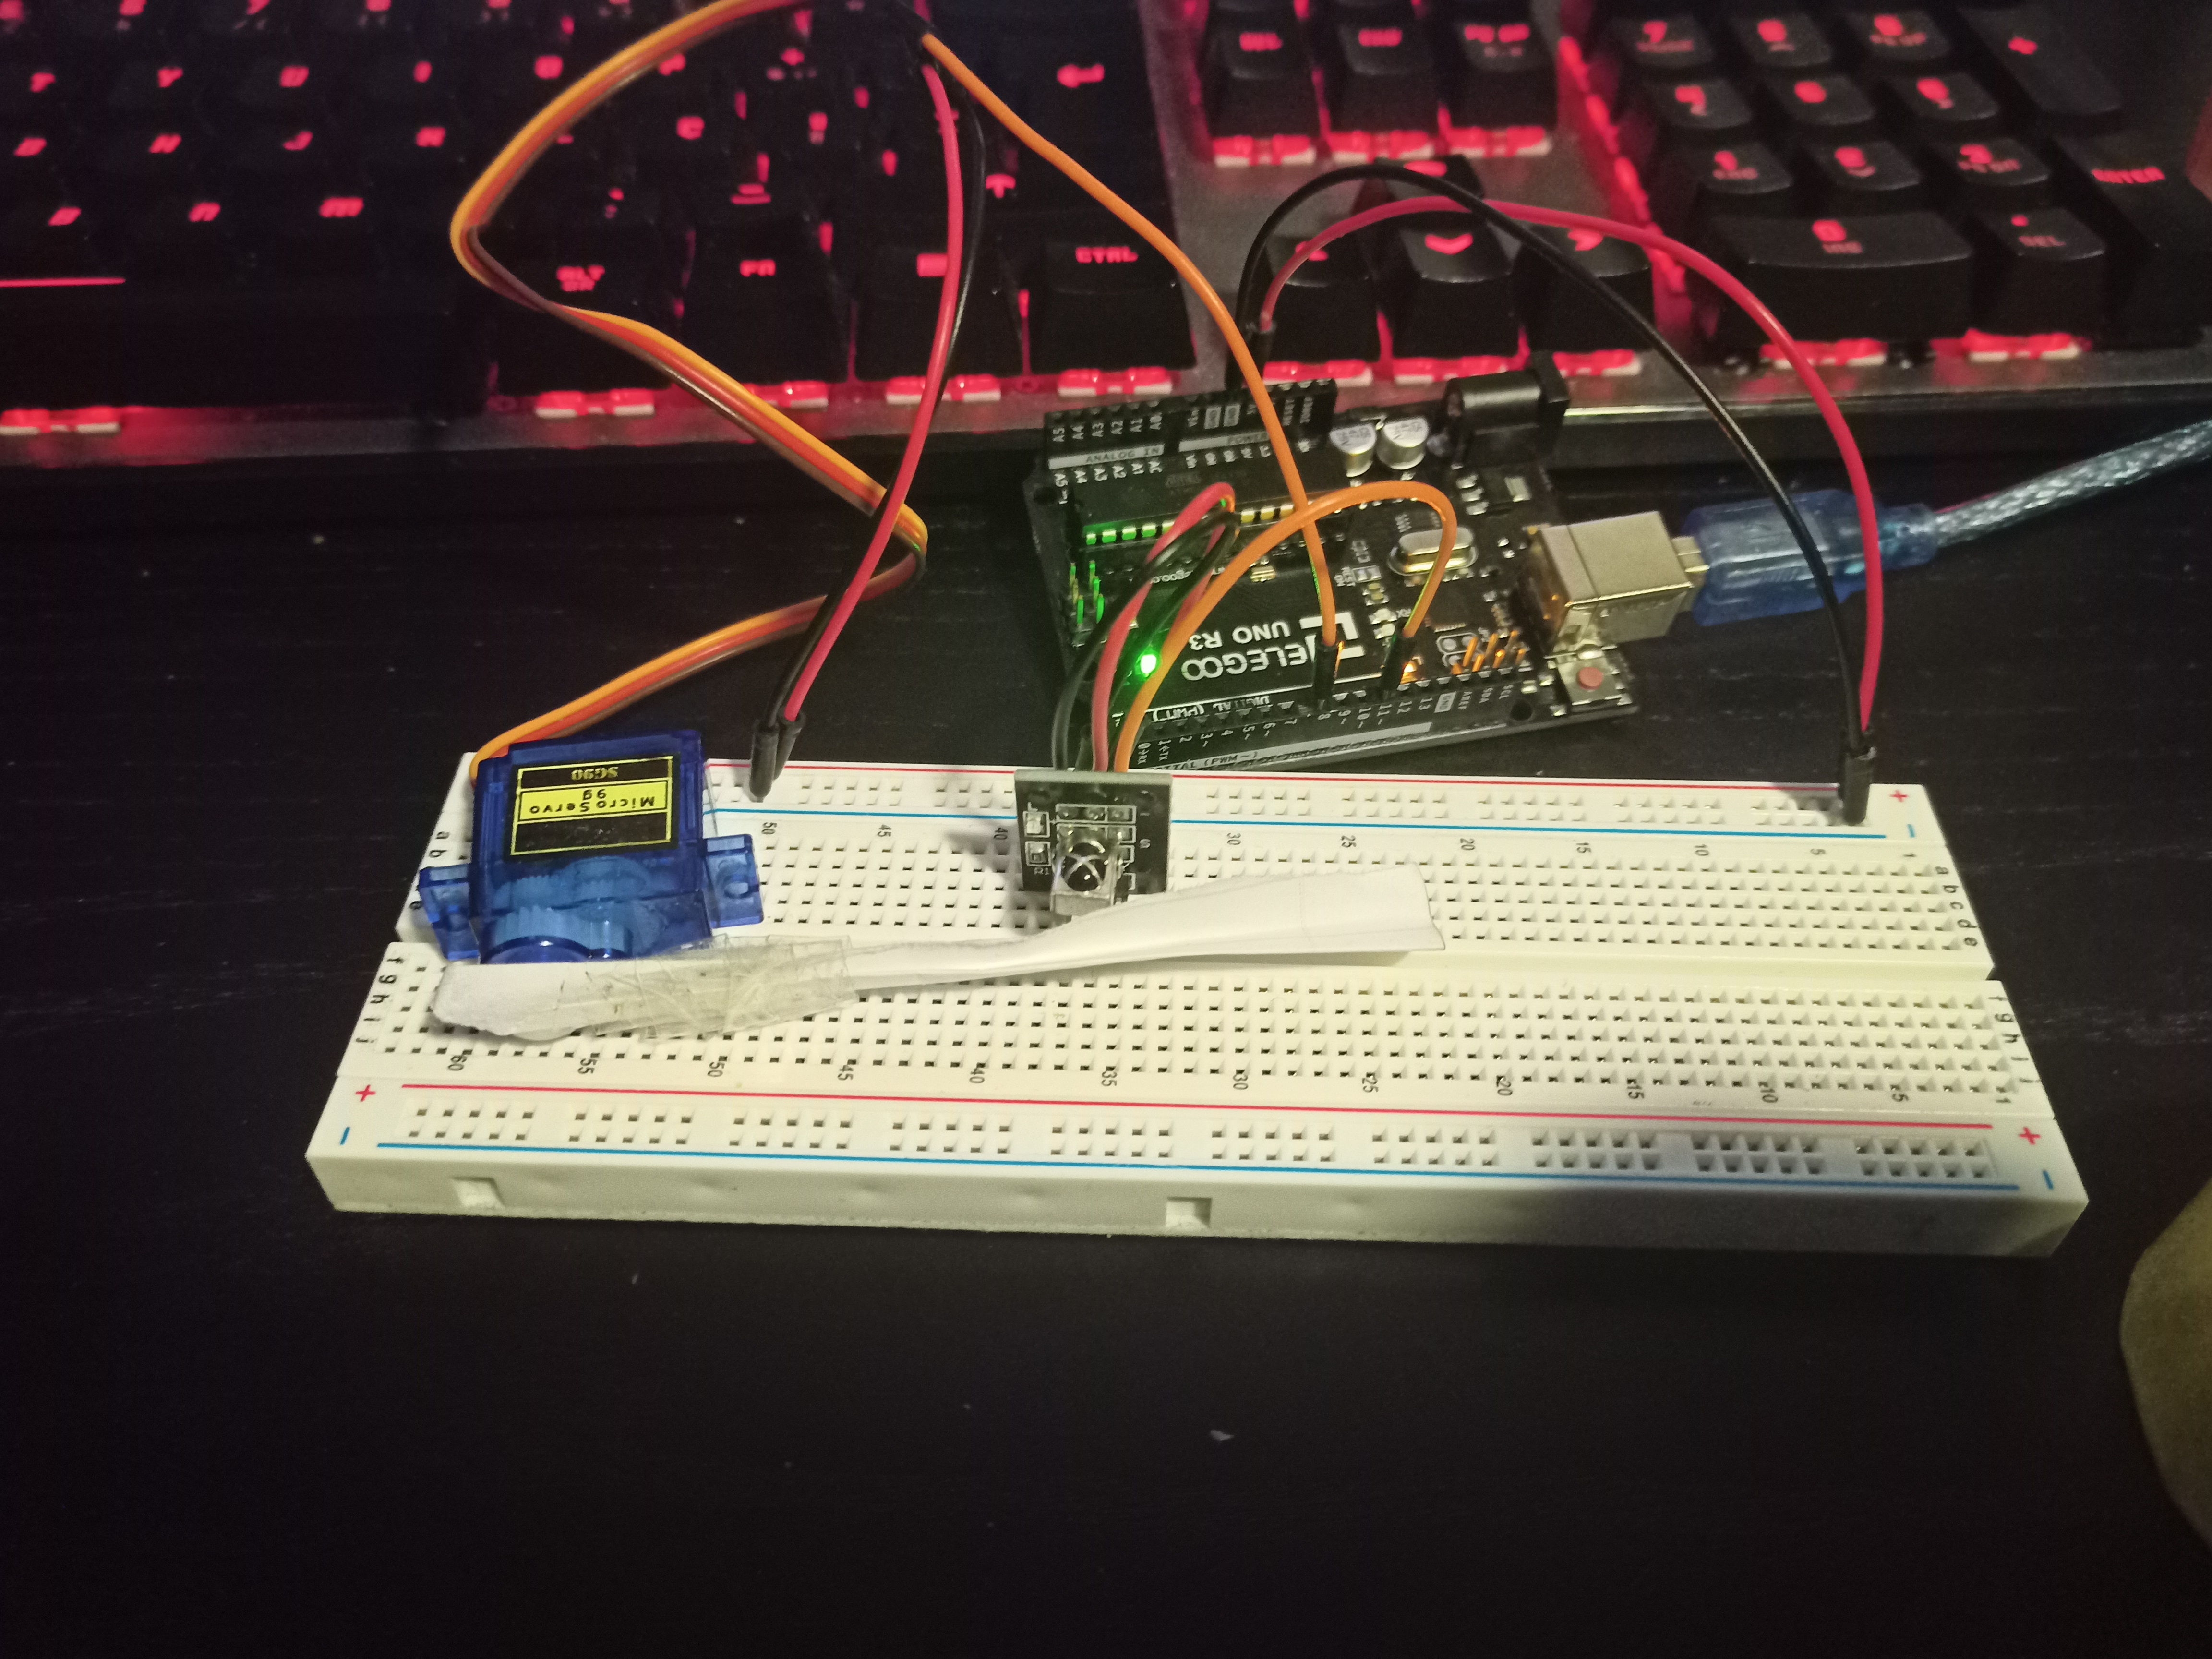
\includegraphics[scale=0.03]{images/testes/sisC_Closed.jpg}
    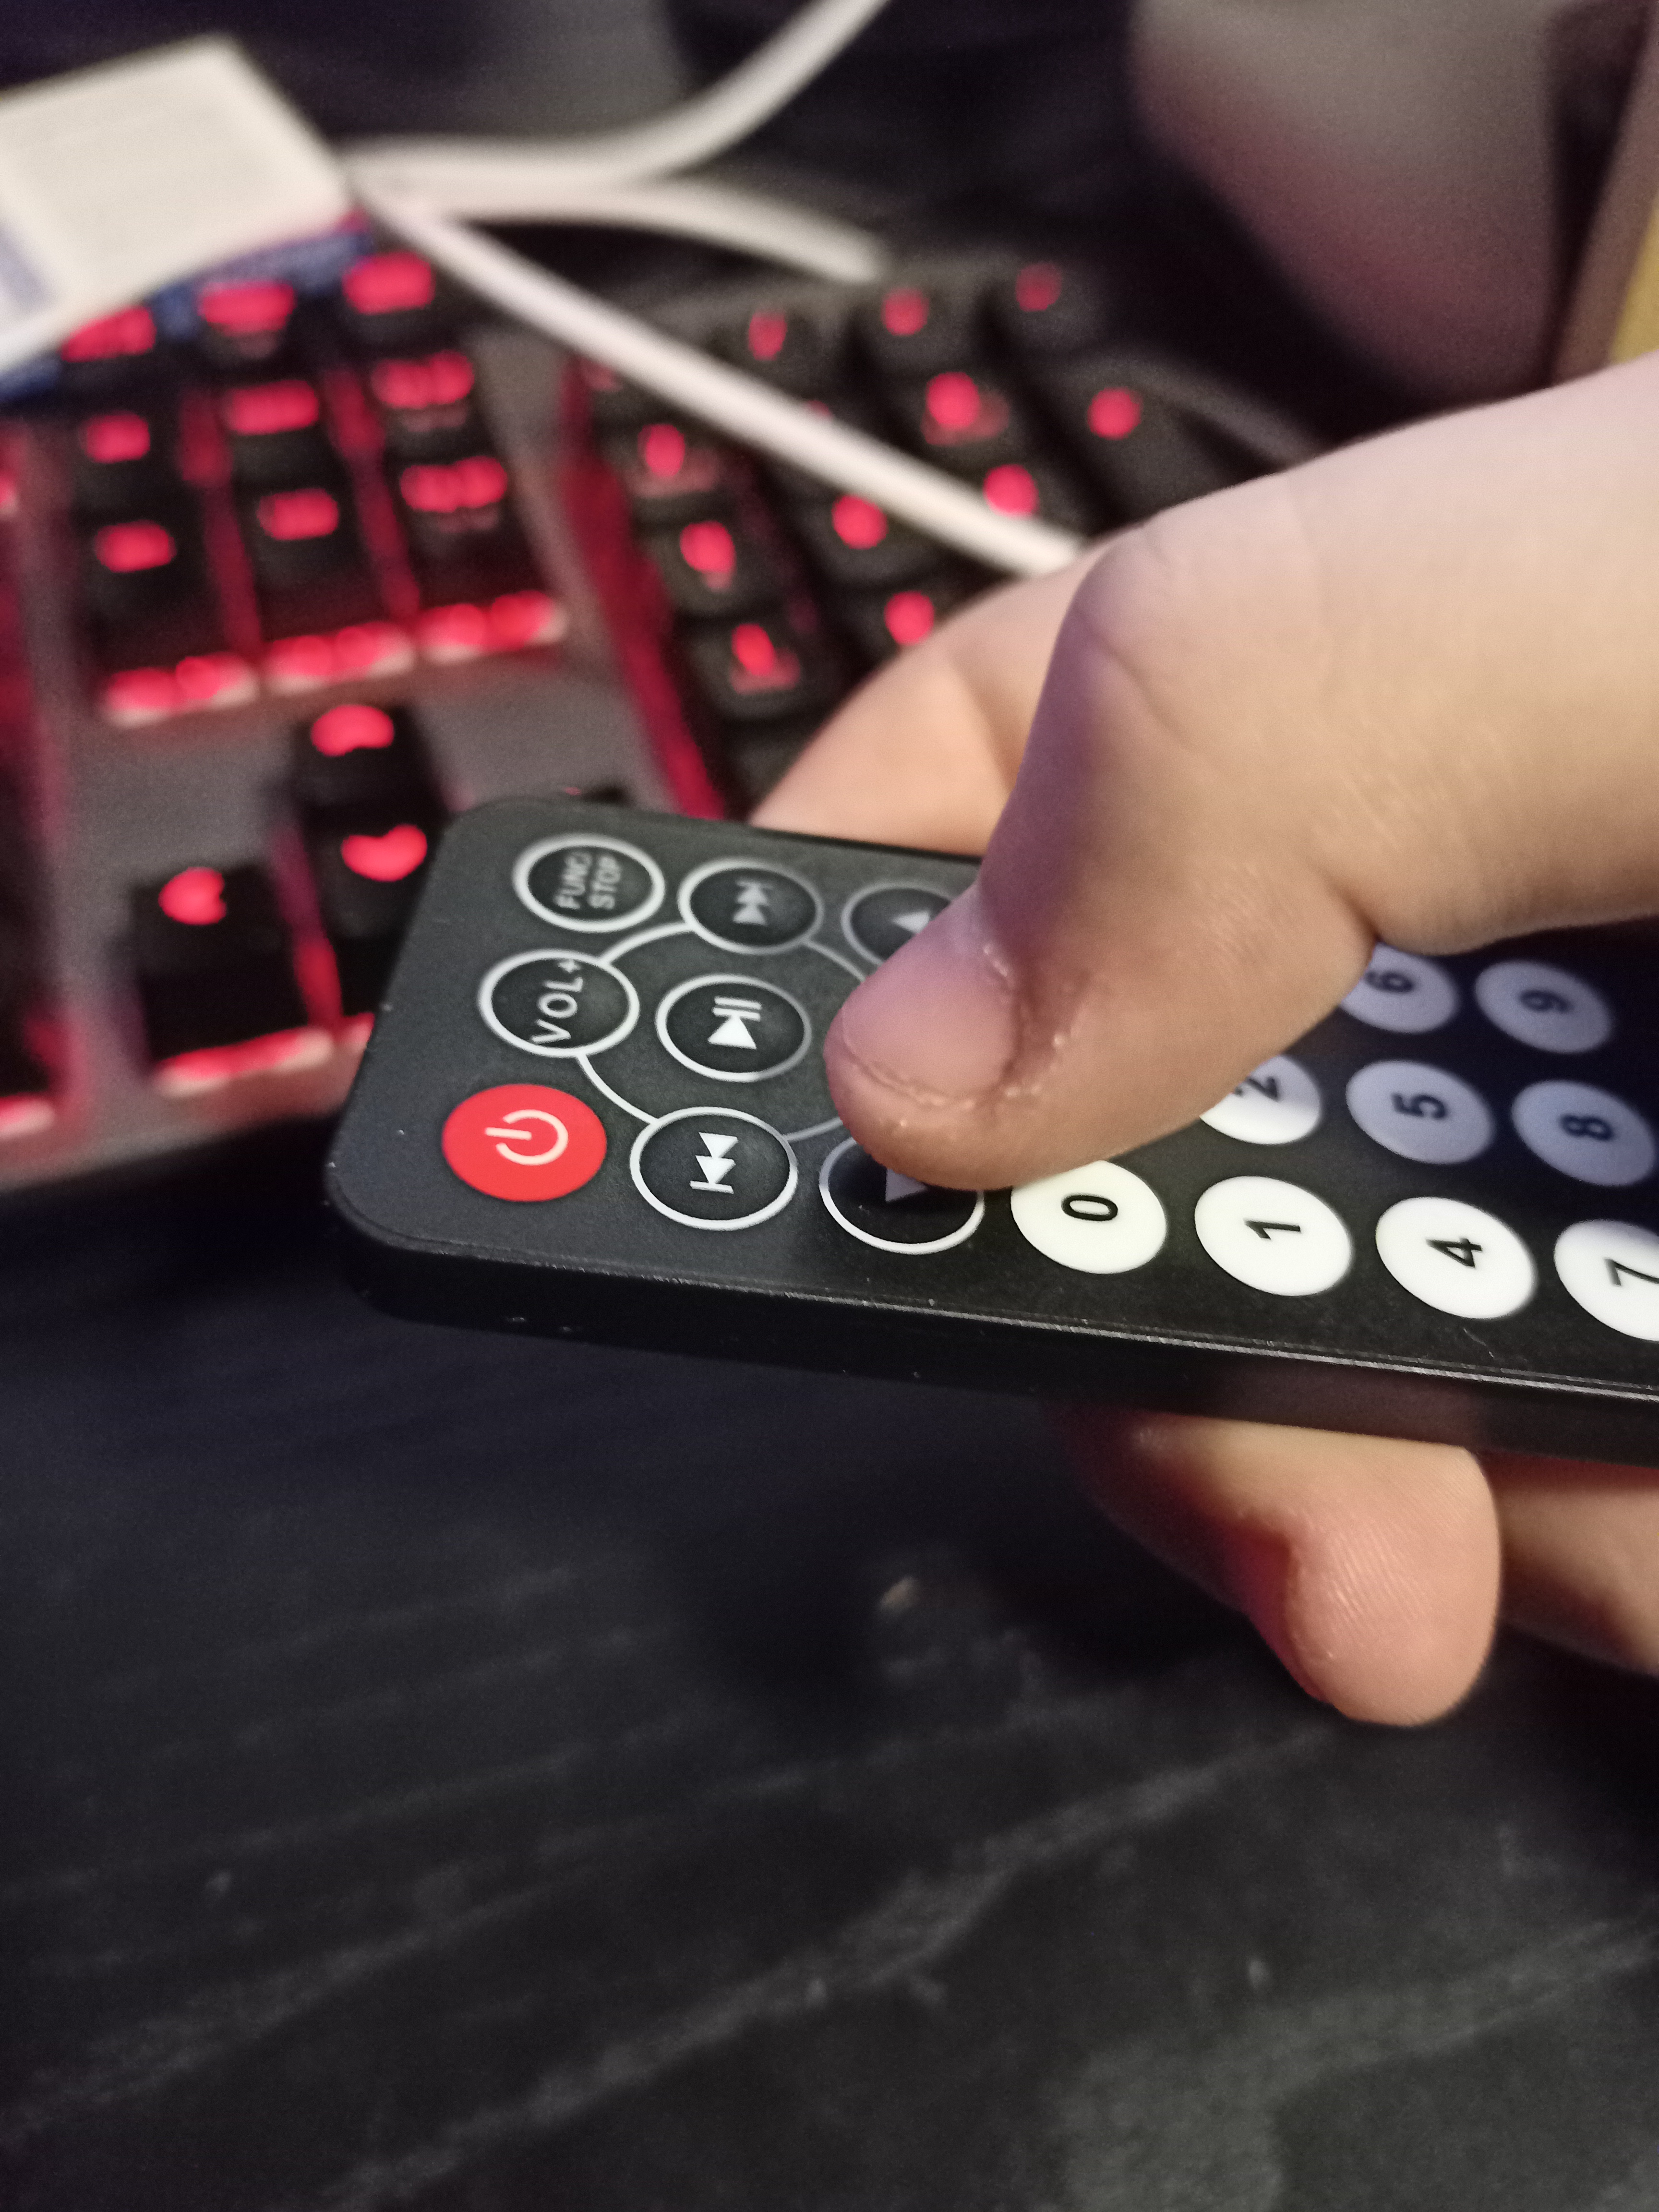
\includegraphics[scale=0.0225]{images/testes/ControllerDown.jpg}
    \selectlanguage{portuguese}\caption{Portão Fechado}
\end{figure}


Foi verificado durante os testes que o sensor de infravermelhos nem sempre deteta os valores corretos do comando. Isto pode ser devido a interferências na corrente, pois a falha na deteção dos códigos é acentuada quando o servo se encontra em movimento.